\Chapter{A járművek mozgásának modellezése}

\Section{Kétkerekű modell kanyarodási íve}

Érdemes lehet előrször a kétkerekű modellt megvizsgálnunk, ugyanis az itt meghatározott képletek adják alapul a négykerekű változatnál használt formulákat. Először is meg kell határoznunk a kanyarodás ívét, ami jelen esetben egy adott elfordulási ($\alpha$) szög mellett tehető meg. Ahogy ez a szög változik úgy fog változni maga az ív is, amin a jármű haladni fog. Ezért első lépésben a sugarat kell megkeresnünk, mert az adott sugárral a középpont köré húzható kör fogja adni az útvonalat. 
A kétkerekű (bicikli) modell kanyarodási ívének meghatározása 2 dologtól függ:\newline
\phantom{len} - a tengelytávolságtól (w),\newline
\phantom{len} - az első kerék kanyarodási szögétől ($\alpha$).\newline
Az első és hátsó kerekek is egy-egy körpályát fognak követni azonos középponttal. Az irány mindig merőleges a sugárra.

\begin{figure}[h!]
\centering
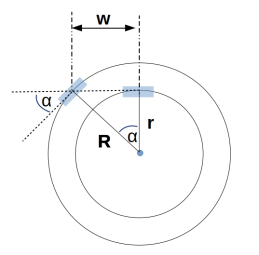
\includegraphics[scale=0.5]{images/two_wheels_rad.png}
\caption{Kétkerekű jármű kanyarodási íve}
\label{fig:two_wheels_rad}
\end{figure}
A \ref{fig:two_wheels_rad} ábrán R az első kerékhez tartozó sugár, r pedig a hátsó kerékhez.\\
Az első kerék pályája: $\sin\alpha$ = $\cfrac{w}{R}$ \hspace{5mm}---> \hspace{5mm} $R$ = $\cfrac{w}{\sin\alpha}$ \\
A hátsó kerék pályája: $\tan\alpha$ = $\cfrac{w}{r}$ \hspace{5mm}---> \hspace{5mm} $r$ = $\cfrac{w}{\tan\alpha}$
\\

Itt a szögfüggvényekben való eltérést a \ref{fig:two_wheels_rad} ábrán látható háromszögől leolvashatjuk, miszerint első kerék esetén a derékszögű háromszög átfogója lesz a sugár, így a kanyarodási szög szinuszát vesszük, a hátsó kerék esetén pedig a szög melletti befogó lesz a sugár, tehát a tangensét kell néznünk. Így átalakítva a képletet megkapjuk a két sugarat.   


\Section{A jármű matematikai modellje}

Áttérve a négykerekű járművekre szintén meg lehet határozni mind a négy kerékhez tartozó sugarat. A \ref{fig:each_wheel_radius}. ábra egy kicsivel részletesebb modellt szemléltet, amin megjelölöm mind a négy sugarat. Az ábrán az úgynevezett Ackerman kanyarodási geometria lényege is látható egy nagyon egyszerű szemléltetéssel, ami megoldja az első két kerék különböző szögekbe való fordítását, ha a jármű fizikai felépítését vesszük. A sugarak kiszámításához képletek a következők:
\\
$R_{IF}$ =  $\cfrac{w}{\sin\alpha_1}$ - $\cfrac{a}{2}$\qquad
$R_{IR}$ =  $\cfrac{w}{\tan\alpha_1}$ - $\cfrac{a}{2}$\\
$R_{OF}$ =  $\cfrac{w}{\sin\alpha_2}$ + $\cfrac{a}{2}$\qquad
$R_{OR}$ =  $\cfrac{w}{\sin\alpha_1}$ + $\cfrac{a}{2}$\\

\begin{figure}[h!]
\centering
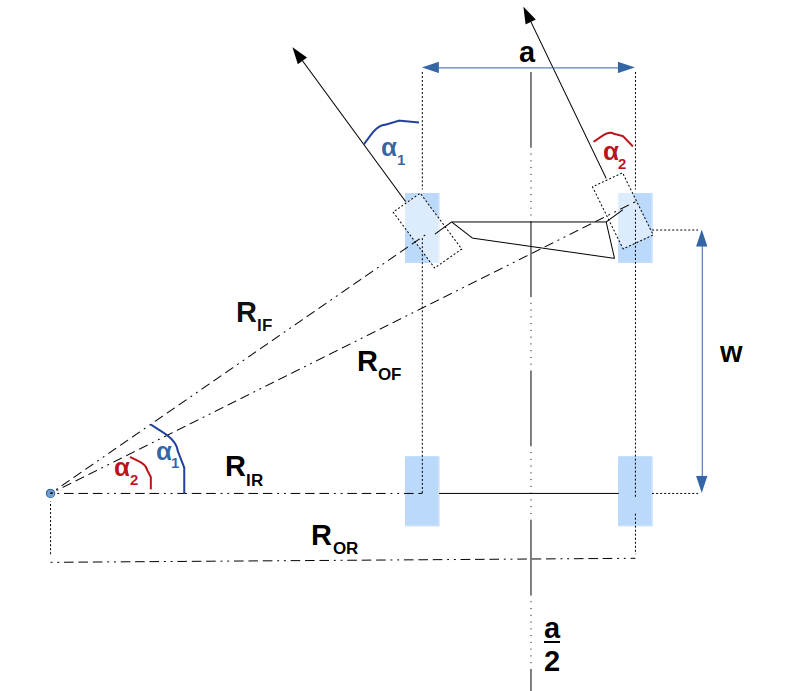
\includegraphics[scale=0.45]{images/each_wheel_radius.png}
\caption{Jármű kerekeinek sugarai}
\label{fig:each_wheel_radius}
\end{figure}

Itt az első kerekeknél a sugár az átfogót képezné, míg a hátsó kerekeknél a szög melletti befogót. Ezért is váltakozik a szinusz és a tangens a trigonometriai összefüggések hatására. Az $\cfrac{a}{2}$ pedig attól függően, hogy a kanyarodás irányához viszonyítva a külső vagy belső kerekekről van szó, a tengely hosszának a felét elvesszük vagy hozzáadjuk a képlethez. 

\subsection{Korábbi technológiák:}

Szeretném egy kicsit részletesebben (kezdetitől a modernebb megoldásokig) bemutatni a jármű modelljét és a kanyarodási elveket/technológiákat. 

A kanyarodás az első kerekek elforgatásával történik. Az első ilyen koncepciónál magát a tengelyt lehetett kormányozni, nem pedig a kerekeket. Ez a megoldás a lassú haladáshoz és a könnyebb manőverezéshez előnyös lehet, de az első tengelynek nagy ívben el kell fordulnia a kanyarodástól függően valamelyik irányba. Ez a futómű kialakítását nagy mértékben korlátozza, maga a felfüggesztés megoldása is nagy kihívás lehet ezt a technológiát alkalmazva.

A kanyarodás következő megoldásánál már mindkét első kerék külön-külön forgatható, de azonos az elfordulási szög. Ebben az esetben a jármű dinamikáját nézve úgynevezett oldal irányú csúszás tapasztalható a kerekeken (a kanyarodás irányának függvényében). Ebben közrejátszik, hogy mivel mindkét kerék egy irányba néz ha el van fordítva a kormány, 2 különböző középpontja lesz a forgásnak, így legalább az egyik kerék csúszni fog a kanyarodáskor.

Ideális megoldásnak vesszük azt az esetet, mikor mindkét első kereket egymástól függetlenül lehet kormányozni. Ebben az esetben mindkét kerék kanyarodási szögét meg lehetne úgy határozni, hogy a kerék középpontja egy érintő egyenes lenne a közös kanyarodási középpontból húzható körívre. Így megválasztva a megfelelő sugarat a körívnek, mindkét kereket tekintve elkerülhető az oldal irányú csúszás. A fejezet további ehhez kapcsolódó pontjai is ezt a megoldást fogják tovább részletezni.\\

Definiálnunk kell különböző jelöléseket, melyek segítségével a képletek leírhatók és értelmezhetők. A négykerekű jármű középpontjának a hátsó tengely középpontját tekintjük. Vagyis esetünkben az elforduláshoz szükséges számításoknál ezt vesszük figyelembe. Mivel a kanyarodásnál az első kerekek különböző szögeket zárnak be az első tengellyel, ezért érdemes egy képzeletbeli, az első tengely közepére eső kormányozható kereket megadni. Ennek a jármű irányával bezárt előjeles szögét jelöljük $\alpha$-val. A jármű tengelytávolságát jelöljük $w$-vel, a hátsó tengely hosszát pedig $a$-val (\ref{fig:vehicle}. ábra).

\begin{figure}[h!]
\centering
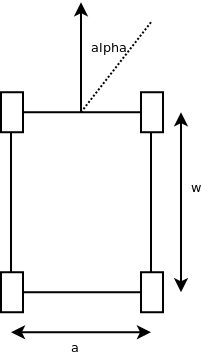
\includegraphics[scale=0.45]{images/vehicle.png}
\caption{A jármű matematikai modelljének fő paraméterei}
\label{fig:vehicle}
\end{figure}

\Section{Első kerekek elfordulási szögének kiszámítása}

A kanyarodásnál tehát figyelembe kell venni, hogy a két első kerék különböző szögben fordul el, mégpedig az iránytól függően a belső kerék nagyobb szögben tér el az egyenestől, míg a külső kisebb szögben. Minél nagyobb a kanyarodási szög, annál nagyobb az eltérés a két kerék elfordulásában.
Az $\alpha$ szög függvényében külön ki kell számítanunk a jármű bal és jobb első kerekének elfordulási szögét.
Tehát első lépésben határozzuk meg az adott $\alpha$ szög ismeretében a további számításokhoz szükséges sugarat,
melyet a \ref{fig:turning_vehicle}. ábrán R jelöl. Ez a kanyarodási sugár, melyet a jármű középvonalához mérünk.
Az ehhez szükséges képlet:\vspace{2mm}
$R$ = $\dfrac{w}{\text{tg} \alpha}$ \vspace{5mm}

Továbbiakban a jelölések ugyanazok, az első kerekeket tekintve pedig $\alpha_1$ a belső, $\alpha_2$ pedig a külső kerék elfordulási szögét jelöli.  
A jármű tengelytávolsága, valamint szélessége, és a sugár ismeretében ezen két szög a következőképpen számítható ki:\vspace{5mm}

$\alpha\textsubscript{1}$ = $\text{arctan}\Bigg(\cfrac{w}{R-\frac{a}{2}}\Bigg)$ \hspace{1cm} $\alpha\textsubscript{2}$ = $\text{arctan}\Bigg(\cfrac{w}{R+\frac{a}{2}}\Bigg)$\vspace{5mm}

\begin{figure}[h!]
\centering
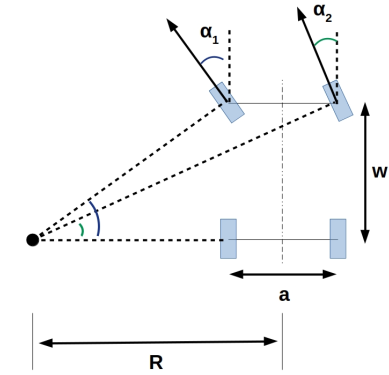
\includegraphics[scale=0.5]{images/turning_vehicle.png}
\caption{Első kerekek elfordulási szögei}
\label{fig:turning_vehicle}
\end{figure}
\vspace{5mm}


A kanyarodási sugárból átalakítható a képlet a trigonometrikus összefüggéseket figyelembe véve. A szögeket megkaphatjuk, ha a képletet rendezzük úgy, hogy a tangens inverzével szorozva elosztjuk a tengelytávolságot az adott kerékhez tartozó sugárral. Ugyanis az arkusz tangens visszaadja azt a szöget, ami jelen esetben a sugárhoz és a tengelytávolsághoz tartozik. Mivel mindkét keréknek más lesz a sugara a kijelölt ponttól, ezeket is külön meg kell határozni, így a képlet nevezőjében a kanyarodási középponthoz közelebb eső kerékhez tartozó sugárból kivonjuk a jármű szélességének felét, míg a messzebb eső kerékhez hozzáadjuk ezt az értéket.

% TODO: Részletesen leírni ezek számítását!

\Section{Pozíció számítása rögzített $\alpha$ mellett}

A rögzített $\alpha$ szög, és adott sebesség mellett ki kell tudnunk számolni, hogy adott $(x_0, y_0)$ kiindulópontból indulva a jármű milyen pozícióba fog kerülni $t$ idő elteltével. Az $\alpha$ szög függvényében az alábbi módon számolhatjuk ki annak a képzeletbeli körnek a sugarát ($R$), amelyen a jármű majd kanyarodni fog:
\[
R = \dfrac{w}{\text{tg} \alpha},
\]
ahol a $w$ a jármű tengelyei közötti távolságot jelöli.

Tegyük fel, hogy a jármű sebessége $v$. Ekkor $t$ idő függvényében a jármű pozícióját az alábbi formában számolhatjuk:
\begin{align*}
x(t) &= x_0 + R - R \cdot \cos \dfrac{v \cdot t}{|R|}, \\
y(t) &= y_0 + |R| \cdot \sin \dfrac{v \cdot t}{|R|}.
\end{align*}

\Section{Útvonal meghatározása az eltelt idő függvényében}

$$
\vec{v} \in \mathbb{R} \hspace{0.5cm}
\quad \rightarrow \quad
\vec{v} (t) \colon \mathbb{R} \to \mathbb{R}^2
$$

Elfordulás:
$$
\varphi (t) \hspace{0.5cm} \rightarrow \hspace{0.5cm} \vec{v} (t) =
\begin{bmatrix}
\cos(\varphi(t)) \\
\sin(\varphi(t))
\end{bmatrix}
$$

$ \vec{x_0} $ : kezdőpozíció

Egy egységnyi idő elteltével az irány: $ \vec{x} (t_1) = \vec{x_0} + \displaystyle\int_{t_0}^{t_1} \vec{v} (t) dt $

Általános alak:  $ \vec{x} (t) = \vec{x_0} + \displaystyle\int_{t_0}^{t} \vec{v} (u) du $

$$
\begin{bmatrix} x_1 \\ y_1 \end{bmatrix} = \begin{bmatrix} x_0 \\ y_0 \end{bmatrix} + \displaystyle\int_{t_0}^{t_1} \begin{bmatrix} \cos(\varphi(t)) \\ \sin(\varphi(t)) \end{bmatrix} dt 
$$


Külön a két vektort leintegráljuk:
\begin{align*}
x_1 &= x_0 + \displaystyle\int_{t_0}^{t_1} \cos(\varphi(t)) \; \mathrm{d}t \\ \\
y_1 &= y_0 + \displaystyle\int_{t_0}^{t_1} \sin(\varphi(t)) \; \mathrm{d}t \\
\end{align*}

Az integrálás kifejtése:
\begin{align*}
x_1 = x_0 + \left[\dfrac{1}{\varphi} \cdot \sin(\varphi(t))\right]_{t_0}^{t_1} = x_0 + \left(\left(\dfrac{1}{\varphi} \cdot \sin(\varphi({t_1)})\right) - \left(\dfrac{1}{\varphi} \cdot \sin(\varphi({t_0}))\right)\right)  \\ \\
y_1 = y_0 + \left[- \dfrac{1}{\varphi} \cdot \cos(\varphi(t))\right]_{t_0}^{t_1} = y_0 + \left(\left(- \dfrac{1}{\varphi} \cdot \cos(\varphi({t_1)})\right) - \left(- \dfrac{1}{\varphi} \cdot \sin(\varphi({t_0}))\right)\right) \\
\end{align*}

Ezzel a számítással megkaphatjuk a jármű által bejárt utat. Jelen esetben a képlet mindig csak a következő pozítiót adja meg, tehát $x_1$ jelentené a következő pozíciót, $x_0$ az előzőt. Az idő szintén a nulladik és az első időpillanatra vonatkozik ($t_0$, $t_1$), valamint a kanyarodási szög mindig az aktuális. Ennek a szögnek az értékénél figyelembe kell venni, hogy negatív vagy pozitív szám. Ez megadja, hogy melyik irányba kanyarodik a jármű a 0 fokhoz képest (ami azt jelenti, hogy előre felé néz). Ha a $\varphi$ < 0 akkor jobbra, ha $\varphi$ > 0  akkor balra fog kanyarodni.

\Section{A jármű mozgása és pozícionálása}

Ebben a pontban szeretném bemutatni a jármű mozgása közben megoldandó pozícionálási problémát. Tehát egy autó-szerű objektumot fogunk vizsgálni, amint megpróbál eljutni egyik pontból a másikba, figyelembe véve azt is, hogy mi a kezdő és végpozíció irányvektora. Továbbra is egy kétdimenziós környezetben fogjuk nézni a jármű mozgását, valamint a kétkerekű modell alapján beállítani a paramétereit. A jármű középpontja a hátsó tengely közepe lesz, így a forgásközéppont a négykerekű járműre illesztett kétkerekű modell hátsó kerekének közepére fog esni. \\\\
Ebben az esetben alapvetően három paraméterrel tudjuk a jármű pozícióját reprezentálni:
\begin{itemize}
	\item x pozíció
	\item y pozíció
	\item $ \delta $ irányszög
\end{itemize}
A számításokhoz a sebességet is figyelembe kell majd venni, ami a jármű pozícióját tekintve x irányban kap értéket, y-ban pedig mindig 0 lesz, ezzel elkerülve az oldal irányú csúszást a kerekek mozgásának megfelelően. A \ref{fig:position} ábrán ezt a részt a szaggatott vonalakkal jelölöm, amik mindig merőlegesek a jármű kerekeire és a forgásközéppontból indulnak. A jármű referenciapontja mindig egy kör alakú pályát követ, aminek a szögsebessége a következő képlettel leírható:\\

$\dot{\delta} = \dfrac{v}{R},$ \\\\
ahol $ v $ a sebesség, $ R $ pedig a hátsó kerék körpályájának a sugara. A későbbiekben $ \gamma $-val jelöljük majd a kanyarodási szöget, ami egy bizonyos értéknél nem lehet nagyobb, tekintve a jármű mechanikáját. Ennek a szögnek a maximum értéke határozza meg a kanyarodási ív sugarának minimális értékét. Egy állandó kanyarodási szög mellett az autó egy körpályán halad, ami miatt a bejárni kívánt út ilyen körívekből épül fel. Tehát minden időpillanatban a kanyarodási szög kis mértékben változik, így az út követése egyszerűbbé válik. Ha egy négykerekű járművet veszünk figyelembe, akkor a kormányzott kerekek különböző sugarú íveket járnak be, és ezzel együtt a két kanyarodó kerék különböző szögekben is fordulnak el. Tehát itt $ \gamma_{inner} $  és $ \gamma_{outer} $ szögeket is meg kell különböztetni, mint a kanyarodás irányát tekintve külső és belső elfordulási szögeket az Ackerman mechanizmus alapján. 
A jármű paraméterei a következő mozgási egyenlet szerint fognak változni:
\begin{itemize}
	\item[] $ \dot{x} = v \cdot \cos\delta $
	\item[] $ \dot{y} = v \cdot \sin\delta $
	\item[] $ \dot{\delta} = \dfrac{v}{L} \cdot \tan\gamma $
\end{itemize}

Melynek $ \dot{\delta} $ értéke a $ \dot{\delta} = \dfrac{v}{R} $ képletből adódik. Ennek geometriai részletezése a metametikai modell résznél található a koncepció fejezetben. 

Ezen modell a kinematikai modellnek felel meg, miszerint a jármű mozgását definiáljuk és nem a járműre ható erőket és egyéb környezeti hatásokat. Maga a pozíció változását a $ \delta $ fogja jelölni ( vagy $ \dot{\delta} $ ), melynek értékét az imént felvezetett irányszög képlete adja. A leírtakat a \ref{fig:position} ábrán keresztül szemléltetem.\\

\begin{figure}[h!]
\centering
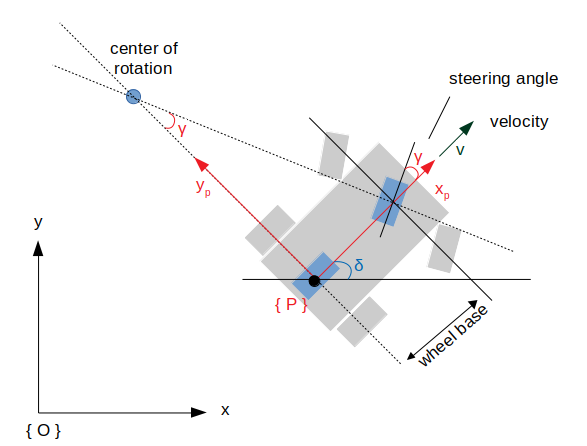
\includegraphics[scale=0.70]{images/position.png}
\caption{A jármű mozgása}
\label{fig:position}
\end{figure}

Az imént felvezetett egyenlet egyéb fontosabb karakterisztikákat is realizál, miszerint $ v = 0-ban$ $ \delta = 0 $, ami azt jelenti, hogy nem tudjuk a jármű orientációját változtatni, ha az nincs mozgásban. Másként: a járműnek muszáj haladnia annak érdekében, hogy fordulni tudjunk vele. 

Ahhoz, hogy el tudjunk mozdulni egy adott pontba, a sebességet arányosan kell változtatni a célhoz való távolság függvényében. Ekkor a következő képletet alkalmazhatjuk:\\

$ v = K \cdot \sqrt{(x\_goal - x)^2 + (y\_goal - y) ^2}$ \\

Valamint a kormányzást a célpozíció felé (ami esetünkben a jármű relatív kanyarodási szögét jelenti) a következő képpen tudjuk definiálni:\\

$ \delta\_goal = \tan^{-1} \cdot \dfrac{y\_goal - y}{x\_goal - x} $\\

valamint a kanyarodási szöget be kell állítani úgy, hogy az a végpontbeli állapot felé irányuljon:\\

$ \gamma = K \cdot ( \delta\_goal \cdot \delta ) $, \qquad ahol $ K > 0 $\\

Így eljutottunk a problémához, hogy a járművet egy bizonyos pozícióba kell irányítani $ (x\_goal, y\_goal, \delta\_goal) $. Az előbbiekben meghatározott képletek segítségével eljuthatunk ebbe a pozícióba a kezdőpozíció ismeretének függvényében. Először is a mozgási egyenletet át kell írnunk mátrix formába, ami a következő képpen fog alakulni:\\

\( \begin{pmatrix}
	\dot{x}\\
	\dot{y}\\
	\dot{\delta}
\end{pmatrix} \)
=
\( \begin{pmatrix}
	\cos\delta & 0\\
	\sin\delta & 0\\
	0 & 1
\end{pmatrix} \)
$ \cdot $ 
\( \begin{pmatrix}
	v\\
	\gamma
\end{pmatrix} \)
\\\\\\
Ezek alapján a ezeket változókat vezethetjük be, hogy irányítani tudjuk a járművet a célban megadott pozíció felé:
\begin{itemize}
	\item[] $ dist = \sqrt{\Delta x^2 + \Delta y^2} $
	\item[] $ \alpha = \tan^{-1} \cdot \dfrac{\Delta y}{\Delta x} - \delta $
	\item[] $ \beta = -\delta - \alpha $
\end{itemize}
 
Ezeket szintén mátrix formába rendezve a következőket kapjuk:\\

\( \begin{pmatrix}
	\dot{dist}\\
	\dot{\alpha}\\
	\dot{\beta}
\end{pmatrix} \)
=
\( \begin{pmatrix}
	\cos\alpha & 0\\\\
	\dfrac{\sin\alpha}{dist} & -1\\\\
	-\dfrac{\sin\alpha}{dist} & 0
\end{pmatrix} \)
$ \cdot $ 
\( \begin{pmatrix}
	v\\
	\gamma
\end{pmatrix} \)
\\\\\\
és feltételezve, hogy a célpozíció a jármű előtt van, az autó irányítása így történik:\\

$ v = K_{dist} \cdot dist $\\

$ \gamma = K_\alpha \cdot \alpha + K_\beta \cdot \beta $\\\\
ahol a konstans értékekre a következő feltételek vonatkoznak: $ K_{dist} > 0, \quad K_\beta < 0, \quad K_\alpha - K_\beta > 0  $\\
Ellenkező esetben ennek az alkalmazott sebességnek a negáltját kell vennünk, tehát tolatni kell a járművel:\\

$ v = -v $, \qquad ha $\alpha \not\in \left(-\dfrac{\pi}{2}, \dfrac{\pi}{2} \right) \quad $ (ez cél szerint változtatható lesz)\\\\
Az lenne a lényege ennek a megoldásnak, hogy a a definiált képletek $ K_{dist} \cdot dist $ és $ K_\alpha \cdot \alpha $ egy vonal mentén vezetik a járművet a cél felé, amíg $ K_\beta \cdot \beta $ ezt a vonalat folyamatosan a cél irányba fordítja.

\begin{figure}[h!]
\centering
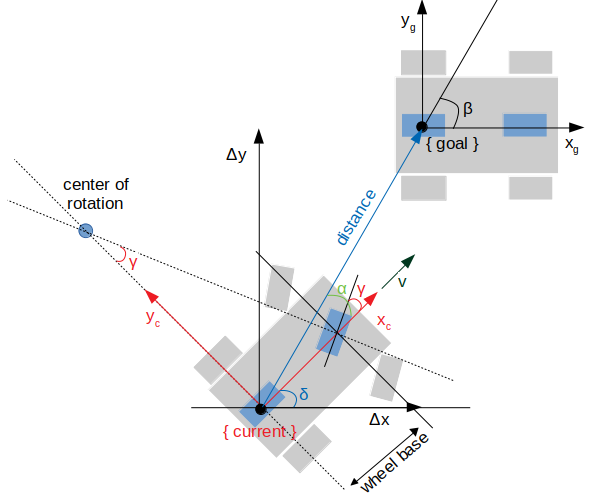
\includegraphics[scale=0.70]{images/moving_vehicle.png}
\caption{A jármű mozgása}
\label{fig:moving_vehicle}
\end{figure}

\subsection{Rotációs mátrix definiálása}

A pozícionáláshoz szükséges pontokat, vektorokat és az azokkal végzett műveleteket szeretném egy kicsit részletezni. Mint már említettem, itt is egy Descartes-féle koordinátarendszerben dolgozunk, melyben egy-egy ponthoz az $ x $ és $ y $ tengely irányába mutató egységvektorok is tartoznak, tehát egy pont így írható le:\\

$ P = x\vec{x} + y\vec{y} $\\\\
Az A-ból B-be való eljutás egyfajta eltolás lesz az A koordinátán. Vagy inkább koordinátarendszeren, mivel a forgatást tekintve a tengelyek, mint vektorok is más-más irányba mutatnak majd. Tehát mondjuk, hogy a B koordináta el lett tolva egy $ t = (x, y) $ vektor által és el lett forgatva egy $ \delta $ szöggel. Ezt a \ref{fig:a_to_b_point} ábra szemlélteti:

\begin{figure}[h!]
\centering
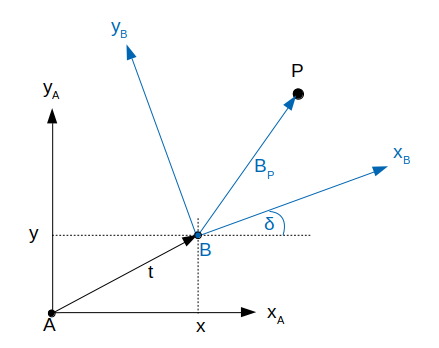
\includegraphics[scale=0.70]{images/A_to_B_point.png}
\caption{A jármű mozgása}
\label{fig:a_to_b_point}
\end{figure}

\newpage

Ha csak a helyzet változást vesszük figyelembe, akkor egy olyan elmozdulást tapasztalunk, amikor a kapott pont tengelyei párhuzamosak a kezdőpontéra. Legyen ez az új pont $ T $, és az imént felírt képlet alapján:\\

$ {}^{T}p = {}^{T}x\vec{x}{}_{T} + {}^{T}y\vec{y}{}_{T} $  =
\(
\begin{pmatrix}
	\vec{x}{}_{T} & \vec{y}{}_{T}
\end{pmatrix}	 
\)
\(
\begin{pmatrix}
	{}^{T}x\\
	{}^{T}y
\end{pmatrix}	 
\)\\\\
A $ B $ pont, már az elforgatást is tartalmazza, mely 2 egység vektorral írható le:\\

$ \vec{x}{}_{B} = \cos\delta\vec{x}{}_{T} + \sin\delta\vec{y}{}_{T} $\\

$ \vec{y}{}_{B} = -\sin\delta\vec{x}{}_{T} + \cos\delta\vec{y}{}_{T} $\\\\
ami mátrix formában felírva a következő:\\

\(
\begin{pmatrix}
	\vec{x}{}_{B} & \vec{y}{}_{B}
\end{pmatrix}
\) =
\(
\begin{pmatrix}
	\vec{x}{}_{T} & \vec{y}{}_{T}
\end{pmatrix}
\)
\(
\begin{pmatrix}
	\cos\delta & -\sin\delta\\
	\sin\delta & \cos\delta
\end{pmatrix}
\)\\\\
A keresett $ P $ pont pedig az előzőekhez hasonlóan felírva:\\

$ {}^{B}p = {}^{B}x\vec{x}{}_{B} + {}^{B}y\vec{y}{}_{B} $  =
\(
\begin{pmatrix}
	\vec{x}{}_{B} & \vec{y}{}_{B}
\end{pmatrix}	 
\)
\(
\begin{pmatrix}
	{}^{B}x\\
	{}^{B}y
\end{pmatrix}	 
\)\\\\
Majd $ B $-vel megszorozva:\\

$ {}^{B}p $ =
\(
	\begin{pmatrix}
		\vec{x}{}_{T} & \vec{y}{}_{T}
	\end{pmatrix}
\)
\(
	\begin{pmatrix}
		\cos\delta & -\sin\delta\\
		\sin\delta & \cos\delta
	\end{pmatrix}
\)
\(
\begin{pmatrix}
	{}^{B}x\\
	{}^{B}y
\end{pmatrix}	 
\)\\\\
Majd a jobb oldali együtthatókat egyenletként felírva a következőt kapjuk:\\

\(
	\begin{pmatrix}
		\vec{x}{}_{T} & \vec{y}{}_{T}
	\end{pmatrix}
\) = 
\(
	\begin{pmatrix}
		\cos\delta & -\sin\delta\\
		\sin\delta & \cos\delta
	\end{pmatrix}
\)
\(
\begin{pmatrix}
	{}^{B}x\\
	{}^{B}y
\end{pmatrix}	 
\qquad \Rightarrow \qquad\)  
\(
	\begin{pmatrix}
		\vec{x}{}_{T} & \vec{y}{}_{T}
	\end{pmatrix}
\) = 
$ {}^{T}R{}_{B} $
\(
\begin{pmatrix}
	{}^{B}x\\
	{}^{B}y
\end{pmatrix}	 
\)\\\\

\begin{figure}[h!]
\centering
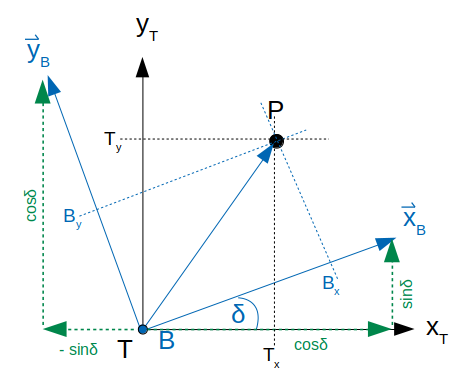
\includegraphics[scale=0.70]{images/T_to_B_point.png}
\caption{A jármű négy pontja a programban}
\label{fig:t_to_b_point}
\end{figure}

És ezzel leírtuk, hogyan forgattuk el a $ T $ pontot a $ B $ pontba. Ez lenne maga a rotációs mátrix. A fent leírt műveleteket a \ref{fig:t_to_b_point} ábra szemlélteti.
\\\\
Ehhez még hozzá kell adnunk az eltolást, ami az $ A $ pontból a $ B $ pontba történik. Ezt egy egyszerű vektoros hozzáadással tehetjük meg:\\


\(
\begin{pmatrix}
	{}^{A}x\\
	{}^{A}y
\end{pmatrix}	 
\) = 
\(
\begin{pmatrix}
	{}^{T}x\\
	{}^{T}y
\end{pmatrix}	 
\) + 
\(
\begin{pmatrix}
	x\\
	y
\end{pmatrix}
\) =
\(
\begin{pmatrix}
	\cos\delta & -\sin\delta\\
	\sin\delta & \cos\delta
\end{pmatrix}
\)
\(
\begin{pmatrix}
	{}^{B}x\\
	{}^{B}y
\end{pmatrix}	 
\) + 
\(
\begin{pmatrix}
	x\\
	y
\end{pmatrix}	 
\)\\\\ = 
\(
	\begin{pmatrix}
		\cos\delta & -\sin\delta & x\\
		\sin\delta & \cos\delta & y
	\end{pmatrix}
\)
\(
\begin{pmatrix}
	{}^{B}x\\
	{}^{B}y\\
	1
\end{pmatrix}	 
\)\\\\
Míg a $2 x 2$ -es mátrix segítségével a forgatást oldottuk meg, magát az elmozdulást egy $ 3 x 3 $ -as adja majd. Egy $t = (x, y) $ vektort fel tudunk írni homogén formában a dimenziószámot egyel növelve, ilyenkor általában egyet adunk meg a harmadik koordinátának. Így a $ P $ pontra vonatkozó transzformációt fel tudjuk írni a következőképpen:\\

$ {}^{A}\vec{p} $ = 
\(
\begin{pmatrix}
	{}^{T}R{}_{B} & t\\
	0_{1x2} & 1
\end{pmatrix}	 
\)
$ {}^{B}\vec{p} $\\\\
Ezek alapján a végső transzformáció:\\

$P(x, y, \delta)$ = 
\(
	\begin{pmatrix}
		\cos\delta & -\sin\delta & x\\
		\sin\delta & \cos\delta & y\\
		0 & 0 & 1
	\end{pmatrix}
\) 
